\section{CTCPNo\-Such\-Service  Class Reference}
\label{classCTCPNoSuchService}\index{CTCPNoSuchService@{CTCPNo\-Such\-Service}}
{\tt \#include $<$CTCPNo\-Such\-Service.h$>$}

Inheritance diagram for CTCPNo\-Such\-Service::\begin{figure}[H]
\begin{center}
\leavevmode
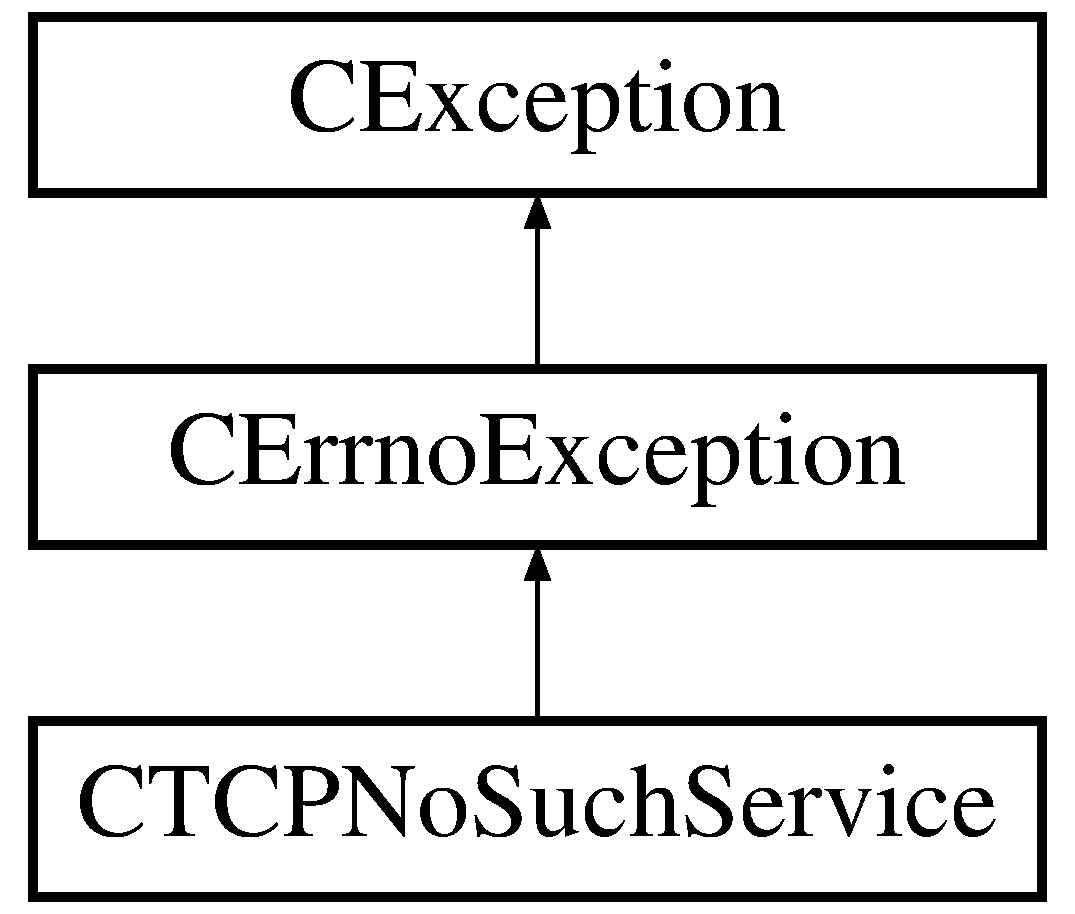
\includegraphics[height=3cm]{classCTCPNoSuchService}
\end{center}
\end{figure}
\subsection*{Public Methods}
\begin{CompactItemize}
\item 
{\bf CTCPNo\-Such\-Service} (const string \&service, const string \&Doing)
\item 
{\bf CTCPNo\-Such\-Service} (const CTCPNo\-Such\-Service \&rhs)
\begin{CompactList}\small\item\em Copy Constructor.\item\end{CompactList}\item 
virtual {\bf $\sim$CTCPNo\-Such\-Service} ()
\begin{CompactList}\small\item\em Destructor.\item\end{CompactList}\item 
CTCPNo\-Such\-Service \& {\bf operator=} (const CTCPNo\-Such\-Service \&rhs)
\item 
int {\bf operator==} (const CTCPNo\-Such\-Service \&rhs)
\item 
string {\bf get\-Service} () const
\begin{CompactList}\small\item\em $<$ Return service name.\item\end{CompactList}\item 
virtual const char $\ast$ {\bf Reason\-Text} () const
\end{CompactItemize}
\subsection*{Protected Methods}
\begin{CompactItemize}
\item 
void {\bf set\-Service} (const string \&new\-Val)
\end{CompactItemize}
\subsection*{Private Attributes}
\begin{CompactItemize}
\item 
string {\bf m\_\-Service}
\begin{CompactList}\small\item\em cached value of service.\item\end{CompactList}\item 
string {\bf m\_\-Reason}
\begin{CompactList}\small\item\em Where the reason text is built up.\item\end{CompactList}\end{CompactItemize}


\subsection{Detailed Description}
Encapsulates an excpetion which indicates a failure to translate a service specification string into a service port number. Service strings can be either a service name which is looked up in e.g. /etc/services or a  stringified service port number. 



Definition at line 309 of file CTCPNo\-Such\-Service.h.

\subsection{Constructor \& Destructor Documentation}
\index{CTCPNoSuchService@{CTCPNo\-Such\-Service}!CTCPNoSuchService@{CTCPNoSuchService}}
\index{CTCPNoSuchService@{CTCPNoSuchService}!CTCPNoSuchService@{CTCPNo\-Such\-Service}}
\subsubsection{\setlength{\rightskip}{0pt plus 5cm}CTCPNo\-Such\-Service::CTCPNo\-Such\-Service (const string \& {\em service}, const string \& {\em Doing})}\label{classCTCPNoSuchService_a0}


Standard constructor. Initialize the member variables to values determined by the application and environmental parameters.\begin{Desc}
\item[Parameters: ]\par
\begin{description}
\item[{\em 
service}]Textualized service which could not be found. This could either be a service name (mis-spelled e.g.) or a textualized service number. \item[{\em 
Doing}]Context information provided by the application to describe what it was trying to do when the failure was detected.\end{description}
\end{Desc}
External inputs:\begin{CompactItemize}
\item 
errno (Thread specific) global variable containing the reason getserv database functions failed. \end{CompactItemize}


Definition at line 309 of file CTCPNo\-Such\-Service.cpp.\index{CTCPNoSuchService@{CTCPNo\-Such\-Service}!CTCPNoSuchService@{CTCPNoSuchService}}
\index{CTCPNoSuchService@{CTCPNoSuchService}!CTCPNoSuchService@{CTCPNo\-Such\-Service}}
\subsubsection{\setlength{\rightskip}{0pt plus 5cm}CTCPNo\-Such\-Service::CTCPNo\-Such\-Service (const CTCPNo\-Such\-Service \& {\em rhs})}\label{classCTCPNoSuchService_a1}


Copy Constructor.

Copy constructor: Creates an object given a reference object. Used by the language to produce temporaries for .e.g. call by value and return by value function interactions.\begin{Desc}
\item[Parameters: ]\par
\begin{description}
\item[{\em 
rhs}]The reference object being copied into $\ast$this. \end{description}
\end{Desc}


Definition at line 322 of file CTCPNo\-Such\-Service.cpp.\index{CTCPNoSuchService@{CTCPNo\-Such\-Service}!~CTCPNoSuchService@{$\sim$CTCPNoSuchService}}
\index{~CTCPNoSuchService@{$\sim$CTCPNoSuchService}!CTCPNoSuchService@{CTCPNo\-Such\-Service}}
\subsubsection{\setlength{\rightskip}{0pt plus 5cm}virtual CTCPNo\-Such\-Service::$\sim$CTCPNo\-Such\-Service ()\hspace{0.3cm}{\tt  [inline, virtual]}}\label{classCTCPNoSuchService_a2}


Destructor.



Definition at line 320 of file CTCPNo\-Such\-Service.h.

\subsection{Member Function Documentation}
\index{CTCPNoSuchService@{CTCPNo\-Such\-Service}!getService@{getService}}
\index{getService@{getService}!CTCPNoSuchService@{CTCPNo\-Such\-Service}}
\subsubsection{\setlength{\rightskip}{0pt plus 5cm}string CTCPNo\-Such\-Service::get\-Service () const\hspace{0.3cm}{\tt  [inline]}}\label{classCTCPNoSuchService_a5}


$<$ Return service name.



Definition at line 328 of file CTCPNo\-Such\-Service.h.

References m\_\-Service.\index{CTCPNoSuchService@{CTCPNo\-Such\-Service}!operator=@{operator=}}
\index{operator=@{operator=}!CTCPNoSuchService@{CTCPNo\-Such\-Service}}
\subsubsection{\setlength{\rightskip}{0pt plus 5cm}CTCPNo\-Such\-Service \& CTCPNo\-Such\-Service::operator= (const CTCPNo\-Such\-Service \& {\em rhs})}\label{classCTCPNoSuchService_a3}


Assignment. Assign $\ast$this to a rhs object. Different from copy construction in that:\begin{CompactItemize}
\item 
We already exist as a validly constructed object.\item 
We return a reference to ourselves so that = chaining is supported.\item 
We prevent self assignment.\end{CompactItemize}
\begin{Desc}
\item[Parameters: ]\par
\begin{description}
\item[{\em 
rhs}]The item to which we are being assigned. \end{description}
\end{Desc}


Definition at line 338 of file CTCPNo\-Such\-Service.cpp.

References m\_\-Service, and CErrno\-Exception::operator=().\index{CTCPNoSuchService@{CTCPNo\-Such\-Service}!operator==@{operator==}}
\index{operator==@{operator==}!CTCPNoSuchService@{CTCPNo\-Such\-Service}}
\subsubsection{\setlength{\rightskip}{0pt plus 5cm}int CTCPNo\-Such\-Service::operator== (const CTCPNo\-Such\-Service \& {\em rhs})}\label{classCTCPNoSuchService_a4}


Equality compare.. This is a field by field compare of the important elements Note that the m\_\-Reason member is unimportant to the compare.\begin{Desc}
\item[Parameters: ]\par
\begin{description}
\item[{\em 
rhs}]The object $\ast$this is being compared to. \end{description}
\end{Desc}


Definition at line 353 of file CTCPNo\-Such\-Service.cpp.

References m\_\-Service, and CErrno\-Exception::operator==().\index{CTCPNoSuchService@{CTCPNo\-Such\-Service}!ReasonText@{ReasonText}}
\index{ReasonText@{ReasonText}!CTCPNoSuchService@{CTCPNo\-Such\-Service}}
\subsubsection{\setlength{\rightskip}{0pt plus 5cm}const char $\ast$ CTCPNo\-Such\-Service::Reason\-Text () const\hspace{0.3cm}{\tt  [virtual]}}\label{classCTCPNoSuchService_a6}


Returns the reason for the exception. This is a string which is built up from CErrno::Reason\-Text and other information we have it is of the form: \char`\"{}Unable to translate service [m\_\-Service] becuase: [CErrno::Reason\-Text()]\char`\"{} 

Reimplemented from {\bf CErrno\-Exception} {\rm (p.\,\pageref{classCErrnoException_a7})}.

Definition at line 367 of file CTCPNo\-Such\-Service.cpp.

References m\_\-Reason, m\_\-Service, and CErrno\-Exception::Reason\-Text().\index{CTCPNoSuchService@{CTCPNo\-Such\-Service}!setService@{setService}}
\index{setService@{setService}!CTCPNoSuchService@{CTCPNo\-Such\-Service}}
\subsubsection{\setlength{\rightskip}{0pt plus 5cm}void CTCPNo\-Such\-Service::set\-Service (const string \& {\em new\-Val})\hspace{0.3cm}{\tt  [inline, protected]}}\label{classCTCPNoSuchService_b0}




Definition at line 334 of file CTCPNo\-Such\-Service.h.

References m\_\-Service.

\subsection{Member Data Documentation}
\index{CTCPNoSuchService@{CTCPNo\-Such\-Service}!m_Reason@{m\_\-Reason}}
\index{m_Reason@{m\_\-Reason}!CTCPNoSuchService@{CTCPNo\-Such\-Service}}
\subsubsection{\setlength{\rightskip}{0pt plus 5cm}string CTCPNo\-Such\-Service::m\_\-Reason\hspace{0.3cm}{\tt  [private]}}\label{classCTCPNoSuchService_o1}


Where the reason text is built up.



Definition at line 314 of file CTCPNo\-Such\-Service.h.

Referenced by Reason\-Text().\index{CTCPNoSuchService@{CTCPNo\-Such\-Service}!m_Service@{m\_\-Service}}
\index{m_Service@{m\_\-Service}!CTCPNoSuchService@{CTCPNo\-Such\-Service}}
\subsubsection{\setlength{\rightskip}{0pt plus 5cm}string CTCPNo\-Such\-Service::m\_\-Service\hspace{0.3cm}{\tt  [private]}}\label{classCTCPNoSuchService_o0}


cached value of service.



Definition at line 313 of file CTCPNo\-Such\-Service.h.

Referenced by get\-Service(), operator=(), operator==(), Reason\-Text(), and set\-Service().

The documentation for this class was generated from the following files:\begin{CompactItemize}
\item 
{\bf CTCPNo\-Such\-Service.h}\item 
{\bf CTCPNo\-Such\-Service.cpp}\end{CompactItemize}
